\documentclass{article}
\usepackage{graphicx}                            % Required for inserting images
\usepackage[paper=a4paper, top=1.5cm, bottom=1.5cm, left=2.0cm, right=2.0cm, heightrounded]{geometry}
\usepackage{hyperref}                            % Clickable links (disabled for minimal TeX install)
\usepackage{array}
\usepackage{multirow}
\usepackage{longtable}
\usepackage{xcolor}
\usepackage{tabularx}
\usepackage{colortbl}
\usepackage{adjustbox}
\usepackage{rotating}
\usepackage{float}
\usepackage[justification=centering]{caption}
\usepackage{listings}
\usepackage{listings}

\usepackage{framed}
\usepackage[nobreak=true]{mdframed}
\usepackage{tikz}
\usepackage{longtable}
\usepackage{pdflscape}
\usepackage{graphicx}
\usepackage{pdfpages}
\usetikzlibrary{positioning, arrows.meta, shapes, calc}

\setlength{\parindent}{0pt}
\setlength{\parskip}{5pt}

\lstdefinelanguage{MyASM}{
  morekeywords={
    SETI, CALL, NOP, RET, SUM, DIF, GTO, SHR, MES, MEL, BNZ
  },
  sensitive=true,
  morecomment=[l]{;},
  morestring=[b]"
}

\lstdefinestyle{asmstyle}{
  language=MyASM,
  basicstyle=\ttfamily\small,
  keywordstyle=\color{blue}\bfseries,
  commentstyle=\color{gray}\itshape,
  stringstyle=\color{red!70!black},
  numbers=left,
  numberstyle=\tiny\color{gray},
  stepnumber=1,
  frame=single,
  rulecolor=\color{black!40},
  backgroundcolor=\color{gray!5},
  tabsize=2,
  showstringspaces=false,
  breaklines=true,
  captionpos=b
}
\graphicspath{ {./img/} }


\lstset{
  basicstyle=\ttfamily\small,      % letra de código
  frame=single,                    % marco alrededor
  columns=fullflexible,
  keepspaces=true,
  showstringspaces=false,
  commentstyle=\color{gray},
  keywordstyle=\color{blue},
  numbers=left,                    % números de línea
  numberstyle=\tiny\color{gray},
  stepnumber=1,
  numbersep=8pt,
  backgroundcolor=\color{gray!10}, % fondo suave
  tabsize=2,
  captionpos=b
}

% Pipeline diagram colors and macros
\newcommand{\IF}{\cellcolor{blue!15}IF}
\newcommand{\ID}{\cellcolor{green!20}ID}
\newcommand{\EX}{\cellcolor{orange!25}EX}
\newcommand{\MEM}{\cellcolor{purple!20}MEM}
\newcommand{\WB}{\cellcolor{gray!20}WB}
\newcommand{\STALL}{\cellcolor{yellow!30}stall}
\newcommand{\FLUSH}{\cellcolor{red!25}flush}

% Text-only stage macros for inline use
\newcommand{\IFtxt}{IF}
\newcommand{\IDtxt}{ID}
\newcommand{\EXtxt}{EX}
\newcommand{\MEMtxt}{MEM}
\newcommand{\WBtxt}{WB}
\newcommand{\STALLtxt}{stall}
\newcommand{\FLUSHtxt}{flush}





\begin{document}


\begin{titlepage}
    \begin{center}
        {\includegraphics[width=0.4\textwidth]{telecomparis.png} \par}
        \vspace{1cm}
        {\bfseries\LARGE Télécom Paris \par}
        \vspace{1cm}
        \vspace{2cm}
        {\scshape\Huge Project 1\par}
        \vspace{1cm}
            {\itshape\Large Execution Platforms \par}
        \vspace{2cm}
        \vfill
        {\Large Members: \par}
        {\Large Barau  Elena\par}
        {\Large Hamdane Brini\par}
        {\Large Marculescu Tudor\par}
        {\Large Wilches Juan\par}
        
        
        \vfill
      
        \vfill
        {\Large January 2026 \par}
    \end{center}
\end{titlepage}
\clearpage


\tableofcontents
\clearpage
\newpage

\section{Introduction to RISC-V Instruction Set Architecture}

In this section we are focusing on a decomposition of RISC-V hex instruction into the ASM instruction.
The instruction format is determined based on the opcode, funct3 and funct7 fields. Table 1 depicts a
detailed translation of each instruction from it's hex code to it's format fields.

\subsection{Program Instructions Decomposition}
\begin{table}[H]
\raggedright
\label{tab:instruction-decomposition}
\vspace{0.3cm}
\renewcommand{\arraystretch}{2}
\begin{adjustbox}{width=\textwidth, center}
\begin{tabular}{|c|c|c|c|c|c|c|c|c|c|c|c|}
\hline
\rowcolor{blue!20}
\textbf{Address} & \textbf{Hex Code} & \textbf{Opcode (6:0)} & \textbf{rd (11:7)} & \textbf{funct3 (14:12)} & \textbf{rs1 (19:15)} & \textbf{rs2 (24:20)} & \textbf{funct7 (31:25)} & \textbf{imm[11:0] (31:20)} & \textbf{imm[X:X] (31:25)} & \textbf{\textbf{imm[X:X] (11:7)}} & \textbf{Type} \\
\hline
0x0  & 0x00050893 & 0010011 & 10001 & 000 & 01010 & - & - & 000000000000 & - & - & I \\
0x4  & 0x00068513 & 0010011 & 01010 & 000 & 01101 & - & - & 000000000000 & - & - & I \\
0x8  & 0x04088063 & 1100011 & - & 000 & 10001 & 00000 & - & - & 0000010 & 00000 & SB \\
0xc  & 0x04058263 & 1100011 & - & 000 & 01011 & 00000 & - & - & 0000010 & 00100 & SB \\
0x10 & 0x04060063 & 1100011 & - & 000 & 01100 & 00000 & - & - & 0000010 & 00000 & SB \\
0x14 & 0x04d05063 & 1100011 & - & 101 & 00000 & 01101 & - & - & 0000010 & 00000 & SB \\
0x18 & 0x00088793 & 0010011 & 01111 & 000 & 10001 & - & - & 000000000000 & - & - & I \\
0x1c & 0x00269713 & 0010011 & 01110 & 001 & 01101 & - & - & 000000000010 & - & - & I \\
0x20 & 0x00e888b3 & 0110011 & 10001 & 000 & 10001 & 01110 & 0000000 & - & 0000000 & 10001 & R \\
0x24 & 0x0007a703 & 0000011 & 01110 & 010 & 01111 & - & - & 000000000000 & - & - & I \\
0x28 & 0x0005a803 & 0000011 & 10000 & 010 & 01011 & - & - & 000000000000 & - & - & I \\
0x2c & 0x01070733 & 0110011 & 01110 & 000 & 01110 & 10000 & 0000000 & - & 0000000 & 01110 & R \\
0x30 & 0x00e62023 & 0100011 & - & 010 & 01100 & 01110 & - & - & 0000000 & 00000 & S \\
0x34 & 0x00478793 & 0010011 & 01111 & 000 & 01111 & - & - & 000000000100 & - & - & I \\
0x38 & 0x00458593 & 0010011 & 01011 & 000 & 01011 & - & - & 000000000100 & - & - & I \\
0x3c & 0x00460613 & 0010011 & 01100 & 000 & 01100 & - & - & 000000000100 & - & - & I \\
0x40 & 0xff1792e3 & 1100011 & - & 001 & 01111 & 10001 & - & - & 1111111 & 00101 & SB \\
0x44 & 0x00008067 & 1100111 & 00000 & 000 & 00001 & - & - & 000000000000 & - & - & I \\
0x48 & 0xfff00513 & 0010011 & 01010 & 000 & 00000 & - & - & 111111111111 & - & - & I \\
0x4c & 0x00008067 & 1100111 & 00000 & 000 & 00001 & - & - & 000000000000 & - & - & I \\
0x50 & 0xfff00513 & 0010011 & 01010 & 000 & 00000 & - & - & 111111111111 & - & - & I \\
0x54 & 0x00008067 & 1100111 & 00000 & 000 & 00001 & - & - & 000000000000 & - & - & I \\
\hline
\end{tabular}
\end{adjustbox}

\vspace{0.2cm}

\footnotesize\textit{Note: Fields marked with dash (-) are not used in the corresponding instruction type. The Type column determines the instruction format: R, I, S, or SB.}
\begin{itemize}
    \setlength\itemsep{0pt}
    \footnotesize\item S-type: imm[X:X] (11:7) = imm[4:0] (11:7) and imm[X:X] (31:25) = imm[11:5] (31:25)
    \footnotesize\item SB-type: imm[X:X] (11:7) = imm[4:1$|$11] (11:7) and imm[X:X] (31:25) = imm[12$|$10:5] (31:25)
\end{itemize}

\caption{Decomposition of Hex Codes to RISC-V Instruction Format}
\end{table}

A point to note is that the immediate fields for UJ and U type instructions are missing from Table 1.
This is because the provided program is missing them. There is also an overlap between the immediates
of S and SB type instructions, as they share the same positions in the instruction format.

\begin{table}[H]
\centering
\label{tab:instructions-simple}
\vspace{0.3cm}
\renewcommand{\arraystretch}{1.6} % Increases row height for all rows
\begin{tabular}{|c|c|c|c|}
\hline
\rowcolor{blue!20}
\textbf{Address} &
\textbf{Hex Code} &
\textbf{ASM Instruction (ABI)} &
\textbf{ASM Instruction (x-registers)} \\
\hline
0x0  & 0x00050893 & addi a7, a0, 0     & addi x17, x10, 0 \\
0x4  & 0x00068513 & addi a0, a3, 0     & addi x10, x13, 0 \\
0x8  & 0x04088063 & beq a7, zero, 64   & beq  x17, x0, 64 \\
0xc  & 0x04058263 & beq a1, zero, 68   & beq  x11, x0, 68 \\
0x10 & 0x04060063 & beq a2, zero, 64   & beq  x12, x0, 64 \\
0x14 & 0x04d05063 & bge zero, a3, 64   & bge  x0, x13, 64 \\
0x18 & 0x00088793 & addi a5, a7, 0     & addi x15, x17, 0 \\
0x1c & 0x00269713 & slli a4, a3, 2     & slli x14, x13, 2 \\
0x20 & 0x00e888b3 & add  a7, a7, a4    & add  x17, x17, x14 \\
0x24 & 0x0007a703 & lw   a4, 0(a5)     & lw   x14, 0(x15) \\
0x28 & 0x0005a803 & lw   a6, 0(a1)     & lw   x16, 0(x11) \\
0x2c & 0x01070733 & add  a4, a4, a6    & add  x14, x14, x16 \\
0x30 & 0x00e62023 & sw   a4, 0(a2)     & sw   x14, 0(x12)   \\
0x34 & 0x00478793 & addi a5, a5, 4     & addi x15, x15, 4   \\
0x38 & 0x00458593 & addi a1, a1, 4     & addi x11, x11, 4   \\
0x3c & 0x00460613 & addi a2, a2, 4     & addi x12, x12, 4   \\
0x40 & 0xff1792e3 & bne a5, a7, -28    & bne  x15, x17, -28 \\
0x44 & 0x00008067 & jalr zero, ra, 0   & jalr x0, x1, 0     \\
0x48 & 0xfff00513 & addi a0, zero, -1  & addi x10, x0, -1   \\
0x4c & 0x00008067 & jalr zero, ra, 0   & jalr x0, x1, 0     \\
0x50 & 0xfff00513 & addi a0, zero, -1  & addi x10, x0, -1   \\
0x54 & 0x00008067 & jalr zero, ra, 0   & jalr x0, x1, 0     \\
\hline
\end{tabular}
\caption{RISC-V Instructions with register numbers, symbolic names and addresses}
\end{table}

In order to better understand the provided program, Table 2 is introduced to map the hex codes with
their corresponding assembly instructions. As an overall view, the program is making use of RV32I instruction
set only. The registers are represented in both their symbolic names (ABI) and x-register numbers.
in order to facilitate the understanding of the program.

\subsection{Branch Delay Slot Concept}
The branch delay slot concept is interesting when discussing pipelined processors. Essentially, when
a branch is taken, instructions fetched after the branch become
invalid if there is no branch prediction mechanism. In early implementations, this issue was handled
by filling the instruction following the branch with a no-operation (NOP) in order to preserve
the normal functioning of the pipeline. However, the problem with this solution is that cycles are wasted doing nothing.

A more efficient approach consists of executing a useful instruction right after the branch (the delay slot).
This instruction is chosen such that it can be executed safely regardless of the branch decision. As a result,
the instruction placed in the delay slot is always executed, whether the branch is taken or not.
This technique helps reduce the performance penalty caused by pipeline flushing after branch instructions.

As explained in \cite{Stack-overflow-branch-delay}: “\textit{The idea of the branch shadow or delay
slot is to recover part of the clock cycles. If the instruction after a branch is always
executed, then when a branch is taken, the instruction in the decode slot is also executed, while
the instruction in the fetch slot is discarded. Therefore, one has a single wasted cycle instead of two.}”
The responsibility of filling the branch delay slot is handled by the compiler during the compilation phase.
To do so, the compiler examines a window of instructions located before and after the branch instruction
and selects an instruction that can be safely moved into the delay slot without changing the program’s behavior.

Figure~\ref{fig:branch_delay_slot} illustrates this behavior in a classical five-stage pipeline (IF, ID, EX, MEM, WB)
using a concrete instruction sequence. In this example, the \texttt{BEQ} instruction is evaluated in the execute stage,
and the branch decision is therefore known only after several cycles. The instruction immediately following the branch,
\texttt{OR r7,r8,r9}, is placed in the delay slot and is executed unconditionally, even when the branch is taken.
In contrast, the subsequent instruction \texttt{XOR r10,r11,r12}, which has already entered the pipeline,
is flushed once the branch outcome is resolved. Execution then continues at the branch target labeled \texttt{Label},
illustrating how the delay slot allows useful work to be performed while limiting the number of wasted cycles.
\begin{figure}[htbp]
\centering
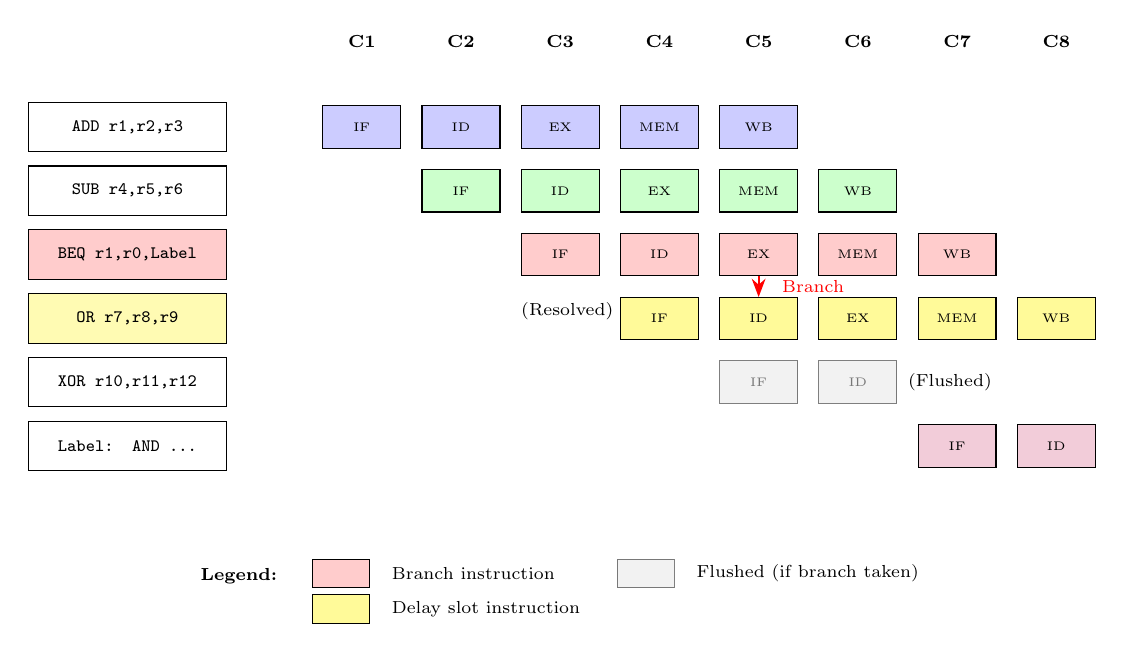
\begin{tikzpicture}[
    scale=0.9,
    transform shape,
    instruction/.style={rectangle, draw, minimum width=2.8cm, minimum height=0.7cm, font=\ttfamily\scriptsize},
    stage/.style={font=\scriptsize\bfseries},
    cycle/.style={font=\scriptsize\bfseries},
    arrow/.style={->, >=Stealth, thick, red}
]

% Cycle numbers at top
\foreach \i in {1,...,8} {
    \node[cycle] at (0.5 + 1.4*\i, 4) {C\i};
}

% Instructions labels on the left
\node[instruction, anchor=east] at (0, 2.8) {ADD r1,r2,r3};
\node[instruction, anchor=east] at (0, 1.9) {SUB r4,r5,r6};
\node[instruction, anchor=east, fill=red!20] at (0, 1.0) {BEQ r1,r0,Label};
\node[instruction, anchor=east, fill=yellow!30] at (0, 0.1) {OR r7,r8,r9};
\node[instruction, anchor=east] at (0, -0.8) {XOR r10,r11,r12};
\node[instruction, anchor=east] at (0, -1.7) {Label: AND ...};

% Pipeline execution boxes with compact spacing
% ADD instruction
\foreach \i/\stage in {1/IF, 2/ID, 3/EX, 4/MEM, 5/WB} {
    \node[draw, fill=blue!20, minimum width=1.1cm, minimum height=0.6cm] at (0.5 + 1.4*\i, 2.8) {\tiny\stage};
}

% SUB instruction
\foreach \i/\stage in {2/IF, 3/ID, 4/EX, 5/MEM, 6/WB} {
    \node[draw, fill=green!20, minimum width=1.1cm, minimum height=0.6cm] at (0.5 + 1.4*\i, 1.9) {\tiny\stage};
}

% BEQ instruction (branch)
\foreach \i/\stage in {3/IF, 4/ID, 5/EX, 6/MEM, 7/WB} {
    \node[draw, fill=red!20, minimum width=1.1cm, minimum height=0.6cm] at (0.5 + 1.4*\i, 1.0) {\tiny\stage};
}

% OR instruction (delay slot - always executed)
\foreach \i/\stage in {4/IF, 5/ID, 6/EX, 7/MEM, 8/WB} {
    \node[draw, fill=yellow!40, minimum width=1.1cm, minimum height=0.6cm] at (0.5 + 1.4*\i, 0.1) {\tiny\stage};
}

% XOR instruction (might be flushed if branch taken)
\foreach \i/\stage in {5/IF, 6/ID} {
    \node[draw, fill=gray!20, minimum width=1.1cm, minimum height=0.6cm, opacity=0.5] at (0.5 + 1.4*\i, -0.8) {\tiny\stage};
}
\node[font=\scriptsize] at (10.2, -0.8) {(Flushed)};

% Target instruction (if branch taken)
\foreach \i/\stage in {7/IF, 8/ID} {
    \node[draw, fill=purple!20, minimum width=1.1cm, minimum height=0.6cm] at (0.5 + 1.4*\i, -1.7) {\tiny\stage};
}

% Arrow showing branch resolution
\draw[arrow] (7.5, 0.7) -- (7.5, 0.4) node[midway, right, font=\scriptsize, xshift=0.2cm] {Branch};
\node[font=\scriptsize] at (4.8, 0.2) {(Resolved)};

% Legend - moved below with branch instruction legend added
\node[font=\scriptsize\bfseries, anchor=north west] at (-0.5, -3.3) {Legend:};

% Branch instruction legend
\node[draw, fill=red!20, minimum width=0.8cm, minimum height=0.4cm, anchor=west] at (1.2, -3.5) {};
\node[font=\scriptsize, anchor=west] at (2.2, -3.5) {Branch instruction};

% Delay slot legend
\node[draw, fill=yellow!40, minimum width=0.8cm, minimum height=0.4cm, anchor=west] at (1.2, -4.0) {};
\node[font=\scriptsize, anchor=west] at (2.2, -4.0) {Delay slot instruction};

% Flushed instruction legend
\node[draw, fill=gray!20, minimum width=0.8cm, minimum height=0.4cm, opacity=0.5, anchor=west] at (5.5, -3.5) {};
\node[font=\scriptsize, anchor=west] at (6.5, -3.5) {Flushed (if branch taken)};

\end{tikzpicture}
\caption{Branch delay slot in a 5-stage pipeline}
\label{fig:branch_delay_slot}
\end{figure}



In terms of advantages and disadvantages, there are several points to consider.

For disadvantages:

\begin{itemize}

\item Branch delay slots may create complications in code debugging, since the instruction in the delay slot
might have side effects, it may lead to an unexpected state of the registers and memory.

\item It adds to the waiting time when trying to execute interruptions, since they will be deffered until
the delay slot instruction is executed. This is a problem in the case of real time systems.

\item Software compatibility requirements dictate that an architecture may not change the number of delay
slots from one generation to the next. This inevitably requires that newer hardware implementations
contain extra components to ensure that the architectural behaviour is followed despite no longer being relevant.
\end{itemize}

Advantages of using branch delay slots include:

\begin{itemize}

\item Improved performance in pipelined architectures, since it helps to reduce the number of pipeline
stalls caused by branch instructions if no branch prediction is used.

\item The use of branch delay slots helps simplify processor design by removing the need for sophisticated
branch prediction mechanisms in early architectures. As a result, the hardware becomes easier and less
expensive to implement.

\end{itemize}

Nowadays, the branch delay slot concept bacame obsolete, as modern processors use branch prediction
techniques to mitigate the braching performance penalty. This also mitigates the complications of
having the compiler finding suitable instructions to fill the delay slots.

\newpage

\subsection{Branch Instructions Analysis}
In order to understand better the provided program, it is useful to check the branch instructions and
where they lead to.

\begin{table}[H]
\centering
\label{tab:instructions-simple}
\vspace{0.3cm}
\renewcommand{\arraystretch}{1.6} % Increases row height for all rows
\begin{tabular}{|c|c|l|}
\hline
\rowcolor{blue!20}
\textbf{Address} & \textbf{Conditional branch} & \textbf{Branch to} \\
\hline

0x08 & beq a7, zero, 64  & 0x48: addi a0, zero, -1 \\
0x0c & beq a1, zero, 68  & 0x50: addi a0, zero, -1 \\
0x10 & beq a2, zero, 64  & 0x50: addi a0, zero, -1 \\
0x14 & bge zero, a3, 148 & 0x54: jalr zero, ra, 0  \\
0x40 & bne a5, a7, -28   & 0x24: lw a4, 0(a5)      \\

\hline
\end{tabular}
\caption{RISC-V Instructions with Addresses}
\end{table}

From the table above we can see that there are 4 first conditional branches, that being the
addresses 0x08, 0x0c, 0x10 and 0x14, which resemble input value checks. Considering the calling
convention for RISC-V, the registers a0-a7 are used for passing function arguments from the caller
to the callee. In this case, the supposition of input value checks is valid. The first three jump
to a return -1 in case the input values are 0, while the fourth one jumps to a return with the number
of elements to be processed, which would be less than or equal to 0.

The last conditional branch at address 0x40 is part of a loop. It checks whether the address stored
in register a5, used as a counter, is equal to the last address to be processed, which is stored in
register a7. If they are not equal, the program branches back to address 0x24 to continue processing
the next elements. If they are equal, the program continues to the return instruction.

\subsection{Program Functionality}

The program can be divided into three main parts: input validation, processing loop, and return value.
The input validation part checks if any of the first three caller arguments are 0. The arguments are
passed are actually pointers to the input and output arrays, so they are checked if they are null,
which would indicate an invalid memory access, therefore leading to a jump to the section of the
program corresponding to return -1. The fourth argument is the number of elements to be processed,
which is checked in the register a3 to see if it is less than or equal to 0. In case it is, the program
jumps to the section corresponding to return, with the number of elements to be processed.

The processing loop starts at address 0x18 and continues until the branch instruction at address 0x40
It consists of an initial setup for the loop counter in register a5 and for the final value of the
counter, which is stored in register a7. Register a7 will store the address of the last element to be processed from
one of the input arrays, calculated as the base address plus the number of elements multiplied by 4,
the size of each element. Because the elements are 4 bytes long, it can be extrapolated that the arrays
are made of 32-bit integers. The loop itself consists of loading the elements from both input arrays,
by using registers a5 and a1, which store the current addresses of the elements. Afterwards, the elements
are summed and stored in register a4, which is then stored in the output array location pointed by register a2.
Finally, the addresses in registers a5, a1 and a2 are incremented by 4 to point to the next elements
to be processed. The loop continues until the address in register a5 is equal to the address in register a7.
This is ensured by the branch if not equal instruction at address 0x40.

Finally, the return part is reached at address 0x44, where the program jumps back to the calle, using
the address stored in register ra. The return value is stored in register a0, which is equal to the
number of elements to be processed.

\begin{table}[H]
\centering
\label{tab:instructions-simple}
\vspace{0.3cm}
\renewcommand{\arraystretch}{1.6} % Increases row height for all rows
\begin{tabular}{|c|c|l|}
\hline
\rowcolor{blue!20}
\textbf{Scenario} & \textbf{Return value} \\
\hline

input pointers are null & -1 \\
number of elements to be processed $\leq$ 0 & number of elemnts to be processed \\
processing finished and the result is ready & number of processed elements      \\

\hline
\end{tabular}
\caption{Return values of the program}
\end{table}

%%%%%%%%%%%%%%%%%%%%%%%%%%%%%%%%%%%%%%%%%%%%%%%%%%%%%%%%%%%%%

% SECTION 2 RISC-V Tool Chain

%%%%%%%%%%%%%%%%%%%%%%%%%%%%%%%%%%%%%%%%%%%%%%%%%%%%%%%%%%%%%


\section{RISC-V Tool Chain}

\subsection {Reimagined C Code}
The above explanation of the program's functionality allows us to reimagine the C code that could
have generated the assembly instructions that were previously described. To do so, one can have an
intuition on what certain assembly instructions would mean. For example, for the part of input
validation, the conditinal branches checks can be equivalent to the if statements of C language.

\begin{mdframed}

    \hspace*{1em} beq a7, zero, 64

    \dots

    addi a0, zero, -1

    jalr zero, ra, 0 $ \longrightarrow $   if (in1 == NULL) return -1;
\end{mdframed}

There is no direct connection between the register names and C variables, therefore arbitrary names
can be assigned to them based on their usage. For example, register a0 can be assigned to the variable
"in1", register a1 to "in2", register a2 to "out" and register a3 to "n", representing the two input
arrays, the output array and the number of elements to be processed from the arrays.

For the processing loop, one can reimagine it as a do while loop, iterating from 0 to n-1. This is
reflected in the assembly instructions which first setup the counter and the final conditional branch
to check if it has reached its final value.

\begin{framed}

    addi a5, a7, 0

    slli a4, a3, 2

    add a7, a7, a4

    \dots

    bne a5, a7, -28 $ \longrightarrow $   in1\_end = in1 + sizeof(int)*n; do \{ \dots \} while (in1 != in1\_end);
\end{framed}

As for the operations inside the loop, the lw can be mapped to array accesses in C, the add instruction
to the assignment operator and the sw to the assignment operator as well.

\begin{framed}
    lw a4, 0(a5)

    lw a6, 0(a1)

    add a4, a4, a6

    sw a4, 0(a2) $ \longrightarrow $   out[i] = in1[i] + in2[i];
\end{framed}

Therefore, taking into account all of the above observations, a complete C functions that could have
generated the provided assembly instructions is represented below:

\begin{lstlisting}[language=C, numbers=left, stepnumber=1, numbersep=5pt]
int addv(int *in1,int *in2,int *out,int n)
{
    if (in1 == NULL)
        return -1;
    if (in2 == NULL)
        return -1;
    if (out == NULL)
        return -1;
    if (n <= 0)
        return n;

    int* in1_end = in1 + sizeof(int)*n;
    do {
        *out = *in1 + *in2;
        in1++;
        in2++;
        out++;
    }
    while (in1 != in1_end);
    return n;
}
\end{lstlisting}

\subsection{Compiling the C Code to RISC-V Assembly}
By using the RISC-V GCC toolchain, one can compile the above C code into RISC-V object code and then
dissasemble it to obtain the assembly instructions. The following command was used in order to produce
the object file "se201-prog.o" from the C source file "se201-prog.c":

\begin{framed}
riscv64-linux-gnu-gcc -g -O0 -mcmodel=medlow -mabi=ilp32 -march=rv32im -Wall -c -o se201-prog.o se201-prog.c
\end{framed}

A fair mention is that in order to have a compilible C program, one needs to provide a main function as
an entry point. In it, the input arrays and the output array are defined, along with the number of
elements to be processed. The call to the addv function, which was seen previously, is also made in
main.


\begin{lstlisting}[language=C, numbers=left, stepnumber=1, numbersep=5pt]
int main() {
    int n = 50;
    int a[50] = {0};
    int b[50] = {0};
    int result[50] = {0};

    addv(a, b, result, n);
    return 0;
}
\end{lstlisting}

\subsection{Comparison between the generated and the previous instructions}

After succefully compiling the C code, one can dissasemble it to obtain the assembly instructions.
The following command is used to do so:

\begin{framed}
riscv64-linux-gnu-objdump -d ./se201-prog.o
\end{framed}

Then, because the addv function is the one of interest, we can navigate to the corresponding part
of the output, containing the label "addv". Below is a snippet of the generated assembly instructions
for it:

Generated Assembly Instructions:
\begin{lstlisting}
00000000 <addv>:
   0:   fd010113                addi    sp,sp,-48
   4:   02812623                sw      s0,44(sp)
   8:   03010413                addi    s0,sp,48
   c:   fca42e23                sw      a0,-36(s0)
  10:   fcb42c23                sw      a1,-40(s0)
  14:   fcc42a23                sw      a2,-44(s0)
  18:   fcd42823                sw      a3,-48(s0)
  1c:   fdc42783                lw      a5,-36(s0)
  20:   00079663                bnez    a5,2c <.L2>
  24:   fff00793                li      a5,-1
  28:   0980006f                j       c0 <.L3>

0000002c <.L2>:
  2c:   fd842783                lw      a5,-40(s0)
  30:   00079663                bnez    a5,3c <.L4>
  34:   fff00793                li      a5,-1
  38:   0880006f                j       c0 <.L3>

0000003c <.L4>:
  3c:   fd442783                lw      a5,-44(s0)
  40:   00079663                bnez    a5,4c <.L5>
  44:   fff00793                li      a5,-1
  48:   0780006f                j       c0 <.L3>

0000004c <.L5>:
  4c:   fd042783                lw      a5,-48(s0)
  50:   00f04663                bgtz    a5,5c <.L6>
  54:   fd042783                lw      a5,-48(s0)
  58:   0680006f                j       c0 <.L3>

0000005c <.L6>:
  5c:   fd042783                lw      a5,-48(s0)
  60:   00479793                slli    a5,a5,0x4
  64:   fdc42703                lw      a4,-36(s0)
  68:   00f707b3                add     a5,a4,a5
  6c:   fef42623                sw      a5,-20(s0)

00000070 <.L7>:
  70:   fdc42783                lw      a5,-36(s0)
  74:   0007a703                lw      a4,0(a5)
  78:   fd842783                lw      a5,-40(s0)
  7c:   0007a783                lw      a5,0(a5)
  80:   00f70733                add     a4,a4,a5
  84:   fd442783                lw      a5,-44(s0)
  88:   00e7a023                sw      a4,0(a5)
  8c:   fdc42783                lw      a5,-36(s0)
  90:   00478793                addi    a5,a5,4
  94:   fcf42e23                sw      a5,-36(s0)
  98:   fd842783                lw      a5,-40(s0)
  9c:   00478793                addi    a5,a5,4
  a0:   fcf42c23                sw      a5,-40(s0)
  a4:   fd442783                lw      a5,-44(s0)
  a8:   00478793                addi    a5,a5,4
  ac:   fcf42a23                sw      a5,-44(s0)
  b0:   fdc42703                lw      a4,-36(s0)
  b4:   fec42783                lw      a5,-20(s0)
  b8:   faf71ce3                bne     a4,a5,70 <.L7>
  bc:   fd042783                lw      a5,-48(s0)

000000c0 <.L3>:
  c0:   00078513                mv      a0,a5
  c4:   02c12403                lw      s0,44(sp)
  c8:   03010113                addi    sp,sp,48
  cc:   00008067                ret
\end{lstlisting}

By comparing the generated assembly with the one provided in the first section, one can observe that
several differences exist. Firstly, the compiler saves the function arguments on the stack before
using them, that being a0, a1, a2 and a3. Then it loads them back from the stack to perform the checks.

Secondly, the check for null pointers, which can be observed in the section from 0x20 -- 0x48 is done
using the "bnez" instruction instead of a "beq", which instead of jumping to a common return -1, they
jump over the return -1 instructions to the next check. This leads to a larger code size and is
also less efficient. The efficiency problem arises from the fact that if bnez is taken, when the pointer
is valid, then the processor will have to flush the pipeline, if no branch prediction is used.

Thirdly, the loop structure is different, as it can be seen in the 0x5c -- 0xb8 section. To compute
the end address of the processing loop, the program first takes out of the stack the value of a3, shifts
it by 4 then adds it to the address of the first element of the array, taken out of the stack as well.
It stores the result back on the stack. In the given assembly, this is done using only three instructions,
without using the stack at all. The same phenomenon can be observed for the loop body, in which each
each element is taken out of the stack, for example the address of the first input array element, which
is used to load the element, then the adress of the second input array element is taken out of the stack
to load the element. They are added and then the address of the output array element is taken out of the
stack to store the result. Finally, the addresses of the of the three arrays can be retaken out of the stack,
incremented by 4 and stored back on the stack.

Finally, the return part is similar, with the difference that actually a ret instruction is used instead
of jalr zero, ra, 0.

\subsection{Changing the Optimization Level}
By switching the optimization level from -O0 to -O, the generated assembly code changes significatly.
It is observed that the code size is reduced, and the loop starts to resemble more the code provided
in the first section. Below is a snippet of the generated assembly instructions:

\begin{lstlisting}
00000000 <addv>:
   0:   00050793                mv      a5,a0
   4:   00068513                mv      a0,a3

00000008 <.LVL1>:
   8:   02078e63                beqz    a5,44 <.L4>
   c:   04058063                beqz    a1,4c <.L5>
  10:   04060263                beqz    a2,54 <.L6>
  14:   04d05263                blez    a3,58 <.L2>
  18:   00469893                slli    a7,a3,0x4
  1c:   011788b3                add     a7,a5,a7

00000020 <.L3>:
  20:   0007a703                lw      a4,0(a5)
  24:   0005a803                lw      a6,0(a1)
  28:   01070733                add     a4,a4,a6
  2c:   00e62023                sw      a4,0(a2)
  30:   00478793                addi    a5,a5,4
  34:   00458593                addi    a1,a1,4

00000038 <.LVL4>:
  38:   00460613                addi    a2,a2,4

0000003c <.LVL5>:
  3c:   fef892e3                bne     a7,a5,20 <.L3>
  40:   00008067                ret

00000044 <.L4>:
  44:   fff00513                li      a0,-1
  48:   00008067                ret

0000004c <.L5>:
  4c:   fff00513                li      a0,-1

00000050 <.LVL8>:
  50:   00008067                ret

00000054 <.L6>:
  54:   fff00513                li      a0,-1

00000058 <.L2>:
  58:   00008067                ret
\end{lstlisting}

Firstly, the stack usage is eliminated completely and the function arguments are used directly from
the registers. Secondly, the input validation part is more efficient, as it uses beqz instructions
that jump directly to the return -1 section. The same phenomenon happens where a5 and a7 are used
as loop counter and address of the last element to be processed, respectively. This version of code
is very similar to the one provided in the first section, with only minor differencces in the return
sections, that use li instead of addi and ret instead of jalr zero, ra, 0.

Changes in code size occur as well when switching to higher optimization levels, such as -O3.

\begin{lstlisting}
00000000 <addv>:
   0:   00050793                mv      a5,a0
   4:   04050063                beqz    a0,44 <.L8>
   8:   02058e63                beqz    a1,44 <.L8>
   c:   02060c63                beqz    a2,44 <.L8>
  10:   00469893                slli    a7,a3,0x4
  14:   011508b3                add     a7,a0,a7
  18:   02d05263                blez    a3,3c <.L5>

0000001c <.L4>:
  1c:   0007a703                lw      a4,0(a5)
  20:   0005a803                lw      a6,0(a1)
  24:   00478793                addi    a5,a5,4

00000028 <.LVL2>:
  28:   00458593                addi    a1,a1,4

0000002c <.LVL3>:
  2c:   01070733                add     a4,a4,a6
  30:   00e62023                sw      a4,0(a2)

00000034 <.LVL4>:
  34:   00460613                addi    a2,a2,4

00000038 <.LVL5>:
  38:   fef892e3                bne     a7,a5,1c <.L4>

0000003c <.L5>:
  3c:   00068513                mv      a0,a3
  40:   00008067                ret

00000044 <.L8>:
  44:   fff00513                li      a0,-1

00000048 <.LVL7>:
  48:   00008067                ret
\end{lstlisting}

Here there are no more output sections that esentially do the same thing, such as in the -O version,
in which the li a0, -1 and ret instructions were repeated three times. The instructions are also
reordered slightly, but the overall structure remains the same.

%%%%%%%%%%%%%%%%%%%%%%%%%%%%%%%%%%%%%%%%%%%%%%%%%%%%%%%%%%%%%%

% SECTION 3 RISC-V Architecture

%%%%%%%%%%%%%%%%%%%%%%%%%%%%%%%%%%%%%%%%%%%%%%%%%%%%%%%%%%%%%%


\section {RISC-V Architecture}

\hspace*{1em} For the following part, a simple RISC-V processor is assumed. It consists of 5 stages Instruction Fetch,
Instruction Decode, Execute, Memory Access and Write Back (IF, ID, EX, MEM, WB).
Register operands are read during the ID stage and written back in the WB stage. The arithmetic operations,
effective address calculations for loads and stores and branch condition evaluation are performed in the
EX stage, while data memory accesses for load and store instructions occur in the MEM stage. The design
forwards ALU results to dependent instructions in order to not stall the pipeline. \cite{patterson-hennessy-cod-riscv}

When a load is consumed immediately by the next instruction, ID inserts a one-cycle stall. \cite{patterson-hennessy-cod-riscv} It is assumed
that the memory replies in one cycle. Branches resolve in EX stage, where when taken, the next two fetched
instructions are flushed and the PC jumps to the branch target. \cite{patterson-hennessy-cod-riscv}

\subsection{Program Flow (5-stage Pipeline)}

\hspace*{1em} Table \ref{tab:program-flow} below presents the complete sequence of instructions executed until the function terminates with a ret instruction. For each instruction, the current architectural state is shown together with a brief explanation of the program behavior. Pipeline hazards, stalls, forwarding events and branch effects are explicitly identified as they occur. \cite{patterson-waterman-riscv-reader}
The table provides a
brief explanation of what happens in the processor and program state. At first the processor has the
registers a0, a1 and a2 set to value 0x200. Register a3 has the value 0x2 and all the other registers
are set to 0.

The memory contents at the addresses 0x200 through 0x210 is given as follows:

\begin{samepage}
\captionsetup{skip=2pt}

\begin{table}[H]
\centering
\label{tab:memory-initial}
\renewcommand{\arraystretch}{1.4}
\begin{tabular}{|c|c|}
\hline
\rowcolor{blue!20}
\textbf{Address} & \textbf{Value} \\
\hline

0x200 & 0x61 \\
0x204 & 0x20 \\
0x208 & 0x62 \\
0x20C & 0x00 \\
0x210 & 0x00 \\
\hline
\end{tabular}
\caption{Initial memory contents}
\end{table}

\vspace{-0.2cm}

\begin{table}[H]
\centering
\renewcommand{\arraystretch}{1.4}
\begin{tabular}{|c|c|}
\hline
\rowcolor{blue!20}
	\textbf{Address} & \textbf{Value} \\
\hline

0x200 & 0xc2 \\
0x204 & 0x40 \\
0x208 & 0x62 \\
0x20C & 0x00 \\
0x210 & 0x00 \\
\hline
\end{tabular}
\caption{Final memory contents after program execution}
\end{table}
\end{samepage}

\newpage
\thispagestyle{empty}
\begin{landscape}
\centering
\setlength{\tabcolsep}{3pt} % Tighten horizontal spacing
\renewcommand{\arraystretch}{1.4} % Professional row spacing

\begin{table}[h]

\label{tab:pipeline-trace}
\resizebox{\linewidth}{!}{%
\begin{tabularx}{1.25\linewidth}{|c|l|c|c|c|c|c|c|c|c|X|X|}
\hline
\rowcolor{blue!20}
\textbf{PC} & \textbf{Instruction} & \textbf{a0} & \textbf{a1} & \textbf{a2} & \textbf{a3} & \textbf{a4} & \textbf{a5} & \textbf{a6} & \textbf{a7} & \textbf{Explanation} & \textbf{Hazard/Resolution} \\
\hline
0x00 & addi a7, a0           & 0x200 & 0x200 & 0x200 & 0x2 & 0x0   & 0x0   & 0x0   & \cellcolor{yellow!25}\textbf{0x200} & Copy value of a0 (return register) into a7 (limit address). & - \\
\hline
0x04 & addi a0, a3           & \cellcolor{yellow!25}\textbf{0x2}   & 0x200 & 0x200 & 0x2 & 0x0   & 0x0   & 0x0   & 0x200 & Copy value of a3 (element count) into a0 (return register). & - \\
\hline
0x08 & beq a7, x0, 0x48      & 0x2   & 0x200 & 0x200 & 0x2 & 0x0   & 0x0   & 0x0   & 0x200 & Branch evaluated in EX stage and found not taken ($R[a7]\neq R[x0]$); normal sequential PC progression, no pipeline flush required. Target: 0x48 = 0x08 + 64. & - \\
\hline
0x0c & beq a1, x0, 0x4c      & 0x2   & 0x200 & 0x200 & 0x2 & 0x0   & 0x0   & 0x0   & 0x200 & Branch evaluated in EX stage and found not taken ($R[a1]\neq R[x0]$); normal sequential PC progression, no pipeline flush required. Target: 0x50 = 0x0c + 68. & - \\
\hline
0x10 & beq a2, x0, 0x50      & 0x2   & 0x200 & 0x200 & 0x2 & 0x0   & 0x0   & 0x0   & 0x200 & Branch evaluated in EX stage and found not taken ($R[a2]\neq R[x0]$); normal sequential PC progression, no pipeline flush required. Target: 0x50 = 0x10 + 64. & - \\
\hline
0x14 & bge x0, a3, 0x54      & 0x2   & 0x200 & 0x200 & 0x2 & 0x0   & 0x0   & 0x0   & 0x200 & Branch evaluated in EX stage and found not taken ($R[x0] < R[a3]$); normal sequential PC progression, no pipeline flush required. Target: 0x54 = 0x14 + 64. & - \\
\hline
0x18 & addi a5, a7, 0        & 0x2   & 0x200 & 0x200 & 0x2 & 0x0   & \cellcolor{yellow!25}\textbf{0x200} & 0x0   & 0x200 & Initialize source pointer: copy value of a7 into a5 (loop cursor). & - \\
\hline
0x1c & slli a4, a3, 2        & 0x2   & 0x200 & 0x200 & 0x2 & \cellcolor{yellow!25}\textbf{0x8}   & 0x200 & 0x0   & 0x200 & Compute byte count for n elements: shift a3 left by 2; value in a4 becomes 8. & - \\
\hline
0x20 & add a7, a7, a4        & 0x2   & 0x200 & 0x200 & 0x2 & 0x8   & 0x200 & 0x0   & \cellcolor{yellow!25}\textbf{0x208} & Compute end pointer: a7 = base + (n*4) = 0x208. & - \\
\hline
0x24 & lw a4, 0(a5)          & 0x2   & 0x200 & 0x200 & 0x2 & \cellcolor{yellow!25}\textbf{0x61}  & 0x200 & 0x0   & 0x208 & Compute address in EX stage (0x200); read word in MEM stage (0x61); write result into a4 in WB. & - \\
\hline
0x28 & lw a6, 0(a1)          & 0x2   & 0x200 & 0x200 & 0x2 & 0x61  & 0x200 & \cellcolor{yellow!25}\textbf{0x61}  & 0x208 & Compute address in EX stage (0x200); read word in MEM stage (0x61); write result into a6 in WB. Next instruction uses a6 immediately, so one cycle stall in ID. & The pipeline encounters a load-use hazard when the next instruction uses a6; the ID stage inserts one stall cycle and then forwards a6 to the EX stage. \\
\hline
0x2c & add a4, a4, a6        & 0x2   & 0x200 & 0x200 & 0x2 & \cellcolor{yellow!25}\textbf{0xc2}  & 0x200 & 0x61  & 0x208 & Add with forwarding: a4 = a4 + a6 = 0xc2. & The forwarding network supplies a6 to the EX stage, so the ALU completes without stalling. \\
\hline
0x30 & sw a4, 0(a2)          & 0x2   & 0x200 & 0x200 & 0x2 & 0xc2  & 0x200 & 0x61  & 0x208 & Compute address in EX stage (0x200); write word in MEM stage (0xc2); memory [0x200] is updated; store uses forwarded a4. & The store uses the forwarded a4 and writes memory without stalling. \\
\hline
0x34 & addi a5, a5, 4        & 0x2   & 0x200 & 0x200 & 0x2 & 0xc2  & \cellcolor{yellow!25}\textbf{0x204} & 0x61  & 0x208 & Advance loop cursor: a5 = a5 + 4. & - \\
\hline
\end{tabularx}%
}
\end{table}
\end{landscape}

\newpage

\thispagestyle{empty}
\begin{landscape}
\centering
\setlength{\tabcolsep}{3pt} % Tighten horizontal spacing for a cleaner look
\renewcommand{\arraystretch}{1.4} % Balanced row height

\begin{table}[h]

\label{tab:program-flow}
\resizebox{\linewidth}{!}{%
\begin{tabularx}{1.15\linewidth}{|c|l|c|c|c|c|c|c|c|c|X|X|}
\hline
\rowcolor{blue!20}
\textbf{PC} & \textbf{Instruction} & \textbf{a0} & \textbf{a1} & \textbf{a2} & \textbf{a3} & \textbf{a4} & \textbf{a5} & \textbf{a6} & \textbf{a7} & \textbf{Explanation} & \textbf{Hazard/Resolution} \\
\hline
0x34 & addi a5, a5, 4        & 0x2   & 0x200 & 0x200 & 0x2 & 0xc2  & \cellcolor{yellow!20}\textbf{0x204} & 0x61  & 0x208 & Advance loop cursor: a5 = a5 + 4. & - \\ \hline
0x38 & addi a1, a1, 4        & 0x2   & \cellcolor{yellow!20}\textbf{0x204} & 0x200 & 0x2 & 0xc2  & 0x204 & 0x61  & 0x208 & Advance source pointer: a1 = a1 + 4. & - \\ \hline
0x3c & addi a2, a2, 4        & 0x2   & 0x204 & \cellcolor{yellow!20}\textbf{0x204} & 0x2 & 0xc2  & 0x204 & 0x61  & 0x208 & Advance destination pointer: a2 = a2 + 4. & - \\ \hline
0x40 & bne a5, a7, -0x1c     & 0x2   & 0x204 & 0x204 & 0x2 & 0xc2  & 0x204 & 0x61  & 0x208 & Branch evaluated in EX stage and found taken ($R[a5]\neq R[a7]$); flush the next two instructions; set PC to 0x24. Target: 0x24 = 0x40 + (-0x1c). & The EX stage takes the branch; the fetch unit flushes two instructions and sets the PC to 0x24. \\ \hline
0x24 & lw a4, 0(a5)          & 0x2   & 0x204 & 0x204 & 0x2 & \cellcolor{yellow!20}\textbf{0x20}  & 0x204 & 0x61  & 0x208 & Compute address in EX stage (0x204); read word in MEM stage (0x20); write result into a4 in WB. & - \\ \hline
0x28 & lw a6, 0(a1)          & 0x2   & 0x204 & 0x204 & 0x2 & 0x20  & 0x204 & \cellcolor{yellow!20}\textbf{0x20}  & 0x208 & Compute address in EX stage (0x204); read word in MEM stage (0x20); write result into a6 in WB. Next instruction uses a6 immediately, so one cycle stall in ID. & The pipeline encounters a load-use hazard when the next instruction uses a6; the ID stage inserts one stall cycle and then forwards a6 to the EX stage. \\ \hline
0x2c & add a4, a4, a6        & 0x2   & 0x204 & 0x204 & 0x2 & \cellcolor{yellow!20}\textbf{0x40}  & 0x204 & 0x20  & 0x208 & Add with forwarding: a4 = a4 + a6 = 0x40. & The forwarding network supplies a6 to the EX stage, so the ALU completes without stalling. \\ \hline
0x30 & sw a4, 0(a2)          & 0x2   & 0x204 & 0x204 & 0x2 & 0x40  & 0x204 & 0x20  & 0x208 & Compute address in EX stage (0x204); write word in MEM stage (0x40); memory [0x204] is updated; store uses forwarded a4. & The store uses the forwarded a4 and writes memory without stalling. \\ \hline
0x34 & addi a5, a5, 4        & 0x2   & 0x204 & 0x204 & 0x2 & 0x40  & \cellcolor{yellow!20}\textbf{0x208} & 0x20  & 0x208 & Advance loop cursor: a5 = a5 + 4. & - \\ \hline
0x38 & addi a1, a1, 4        & 0x2   & \cellcolor{yellow!20}\textbf{0x208} & 0x204 & 0x2 & 0x40  & 0x208 & 0x20  & 0x208 & Advance source pointer: a1 = a1 + 4. & - \\ \hline
0x3c & addi a2, a2, 4        & 0x2   & 0x208 & \cellcolor{yellow!20}\textbf{0x208} & 0x2 & 0x40  & 0x208 & 0x20  & 0x208 & Advance destination pointer: a2 = a2 + 4. & - \\ \hline
0x40 & bne a5, a7, -0x1c     & 0x2   & 0x208 & 0x208 & 0x2 & 0x40  & 0x208 & 0x20  & 0x208 & Branch evaluated in EX stage and found not taken ($R[a5]= R[a7]$); normal sequential PC progression, no pipeline flush required. Target: 0x24 = 0x40 + (-0x1c), not taken. & The EX stage resolves the branch as not taken; the PC advances sequentially and no flush occurs. \\ \hline
0x44 & ret                   & 0x2   & 0x208 & 0x208 & 0x2 & 0x40  & 0x208 & 0x20  & 0x208 & Return to \texttt{ra}; a0 already holds the element count (n=0x2). & - \\ \hline
\end{tabularx}%
}
\caption{Program flow with pipeline notes and hazards (changed registers highlighted)}
\end{table}

\end{landscape}

\newpage
Note: In the actual code, \texttt{jalr zero, ra, 0} encodes the \texttt{ret} pseudoinstruction, returning to the address held in \texttt{ra}.

\subsection{Pipeline Diagram}
\noindent The following diagrams show the 5-stage pipeline progression for all executed instructions. Colors denote pipeline stages; stalls and flushed wrong-path instructions are highlighted.




\begin{center}

\setlength{\tabcolsep}{12pt} % Balanced spacing for a legend
\renewcommand{\arraystretch}{2.0} % Generous height for clarity

\begin{table}[h]
\centering

\label{tab:stage-legend}
\begin{tabularx}{\linewidth}{|l|l|X|}
\hline
\rowcolor{blue!20}
\textbf{Stage} & \textbf{Color} & \textbf{Role and Notes} \\
\hline
Instruction Fetch & \IF & Fetches the instruction at the current PC; sequentially increments PC unless a taken branch in \EXtxt \ overrides it. Wrong-path instructions after a taken branch become \FLUSHtxt. \\
\hline
Instruction Decode & \ID & Reads source registers and decodes opcode; detects hazards. On a load-use dependency, \IDtxt \ inserts a single \STALLtxt \ bubble before the dependent instruction can enter \EXtxt. \\
\hline
Execute & \EX & Performs ALU operations, effective address calculation, and branch resolution. Forwarding supplies operands from prior \EXtxt/\MEMtxt \ results to avoid stalls for ALU dependencies. \\
\hline
Memory & \MEM & Reads or writes data memory for loads/stores using the effective address computed in \EXtxt. Load results are available for forwarding after \MEMtxt. \\
\hline
Writeback & \WB & Writes results to destination registers (for ALU and loads). Stores do not write back. \\
\hline
Stall & \STALL & Represents a bubble introduced to wait for data (e.g. after a load when the very next instruction consumes the loaded value). \\
\hline
Flush & \FLUSH & Marks wrong-path instructions fetched before a taken branch resolves in \EXtxt; these do not affect architectural state. \\
\hline
\end{tabularx}
\caption{Pipeline Stage Descriptions and Role Definitions}
\end{table}
\end{center}


\vspace{0.3cm}


\noindent \textbf{Pipeline Overview}\\
\indent The processor uses a classic five-stage in-order pipeline. Instructions advance one stage per cycle unless a hazard forces a stall or a taken branch flushes wrong-path work.\par
\indent Forwarding sends ALU results from \EXtxt \ and \MEMtxt \ to subsequent instructions, allowing dependent additions (e.g. \texttt{add a4,a4,a6}) to proceed without stalling. \cite{patterson-hennessy-cod-riscv}\par
\indent A load-use hazard occurs when the very next instruction needs a loaded value (\texttt{lw} immediately followed by \texttt{add}). The \IDtxt \ stage inserts a one-cycle \STALLtxt \ so that \MEMtxt \ can produce the value and the result is then forwarded into \EXtxt. \par
\indent Branch resolution happens in \EXtxt. When the branch is taken, the fetch unit flushes the next two wrong-path instructions and redirects the PC to the computed target. When the branch is not taken, the PC advances sequentially. \cite{patterson-hennessy-cod-riscv}\par
\indent Stores consume forwarded data (e.g. the new \texttt{a4} value) and update memory in \MEMtxt. They do not introduce additional stalls in this design.\par
\indent In the diagrams, each row shows an instruction’s stages by cycle (C1, C2, …). \STALLtxt cells indicate bubbles that are inserted and \FLUSHtxt rows show wrong-path instructions that are discarded after a taken branch.
\vspace{0.2cm}


\noindent \textbf{Setup (PC 0x00–0x20)}\\[0pt]
\noindent
\renewcommand{\arraystretch}{1.3}
\begin{table}[H]
\centering
\begin{adjustbox}{width=\textwidth, center}
\begin{tabular}{|l|c|c|c|c|c|c|c|c|c|c|c|c|}
\hline
\rowcolor{blue!20}
Instruction & C1 & C2 & C3 & C4 & C5 & C6 & C7 & C8 & C9 & C10 & C11 & C12 \\
\hline
0x00 addi a7,a0 & \IF & \ID & \EX & \MEM & \WB &  &  &  &  &  &  &  \\
0x04 addi a0,a3 &  & \IF & \ID & \EX & \MEM & \WB &  &  &  &  &  &  \\
0x08 beq a7,zero,64 (NT) &  &  & \IF & \ID & \EX &  &  &  &  &  &  &  \\
0x0c beq a1,zero,68 (NT) &  &  &  & \IF & \ID & \EX &  &  &  &  &  &  \\
0x10 beq a2,zero,64 (NT) &  &  &  &  & \IF & \ID & \EX &  &  &  &  &  \\
0x14 bge zero,a3,64 (NT) &  &  &  &  &  & \IF & \ID & \EX &  &  &  &  \\
0x18 addi a5,a7,0 &  &  &  &  &  &  & \IF & \ID & \EX & \MEM & \WB &  \\
0x1c slli a4,a3,2 &  &  &  &  &  &  &  & \IF & \ID & \EX & \MEM & \WB \\
0x20 add a7,a7,a4 &  &  &  &  &  &  &  &  & \IF & \ID & \EX & \MEM \\
\hline
\end{tabular}
\end{adjustbox}
\caption{Setup pipeline overview (PC 0x00–0x20): initial instructions advance without stalls; establishes pointers and byte count for the loop.}
\label{tab:pipeline-setup}
\end{table}

\vspace{0.4cm}
\noindent \textbf{Iteration 1 (PC 0x24–0x40, branch taken)}\\[0pt]
\noindent
\begin{table}[H]
\centering
\begin{adjustbox}{width=\textwidth, center}
\begin{tabular}{|l|c|c|c|c|c|c|c|c|c|c|c|}
\hline
\rowcolor{blue!20}
Instruction & C1 & C2 & C3 & C4 & C5 & C6 & C7 & C8 & C9 & C10 & C11 \\
\hline
0x24 lw a4,0(a5) & \IF & \ID & \EX & \MEM & \WB &  &  &  &  &  &  \\
0x28 lw a6,0(a1) &  & \IF & \ID & \EX & \MEM & \WB &  &  &  &  &  \\
0x2c add a4,a4,a6 &  &  & \IF & \ID & \STALL & \EX (\cellcolor{orange!25}EX\,\textit{fwd}) & \MEM & \WB &  &  &  \\
0x30 sw a4,0(a2) &  &  &  & \IF & \ID & \EX & \MEM &  &  &  &  \\
0x34 addi a5,4 &  &  &  &  & \IF & \ID & \EX & \MEM & \WB &  &  \\
0x38 addi a1,4 &  &  &  &  &  & \IF & \ID & \EX & \MEM & \WB &  \\
0x3c addi a2,4 &  &  &  &  &  &  & \IF & \ID & \EX & \MEM & \WB \\
0x40 bne a5,a7,-28 (T) &  &  &  &  &  &  &  & \IF & \ID & \EX (\cellcolor{orange!25}EX\,\textit{branch}) &  \\
0x44 ret (flushed) &  &  &  &  &  &  &  &  & \IF & \FLUSH &  \\
0x48 addi a0,-1 (flushed) &  &  &  &  &  &  &  &  &  & \IF & \FLUSH \\
\hline
\end{tabular}
\end{adjustbox}
\caption{Iteration 1 pipeline overview (branch taken): shows load-use stall and forwarding into add; store updates memory; branch resolves taken and flushes wrong-path instructions.}
\label{tab:pipeline-iter1}
\end{table}



\vspace{0.4cm}
\noindent \textbf{Iteration 2 and return (PC 0x24–0x44, branch not taken)}\\[0pt]
\noindent
\begin{table}[H]
\centering
\begin{adjustbox}{width=\textwidth, center}
\begin{tabular}{|l|c|c|c|c|c|c|c|c|c|c|c|c|}
\hline
\rowcolor{blue!20}
Instruction & C1 & C2 & C3 & C4 & C5 & C6 & C7 & C8 & C9 & C10 & C11 & C12 \\
\hline
0x24 lw a4,0(a5) & \IF & \ID & \EX & \MEM & \WB &  &  &  &  &  &  &  \\
0x28 lw a6,0(a1) &  & \IF & \ID & \EX & \MEM & \WB &  &  &  &  &  &  \\
0x2c add a4,a4,a6 &  &  & \IF & \ID & \STALL & \EX (\cellcolor{orange!25}EX\,\textit{fwd}) & \MEM & \WB &  &  &  &  \\
0x30 sw a4,0(a2) &  &  &  & \IF & \ID & \EX & \MEM &  &  &  &  &  \\
0x34 addi a5,4 &  &  &  &  & \IF & \ID & \EX & \MEM & \WB &  &  &  \\
0x38 addi a1,4 &  &  &  &  &  & \IF & \ID & \EX & \MEM & \WB &  &  \\
0x3c addi a2,4 &  &  &  &  &  &  & \IF & \ID & \EX & \MEM & \WB &  \\
0x40 bne a5,a7,-28 (NT) &  &  &  &  &  &  &  & \IF & \ID & \EX (\cellcolor{orange!25}EX\,\textit{branch}) &  &  \\
0x44 ret &  &  &  &  &  &  &  &  & \IF & \ID & \EX & \WB \\
\hline
\end{tabular}
\end{adjustbox}
\caption{Iteration 2 pipeline overview (branch not taken): repeats the sequence with forwarding; branch resolves not taken; execution returns without additional flushes.}
\label{tab:pipeline-iter2}
\end{table}


\newpage
\section {Procressor Design}
\subsection {Instruction Set Architecture}


The processor designed in this project uses a fixed instruction width of 16 bits.
It includes 16 general-purpose registers, each 32 bits wide, allowing operations on 32-bit data values.

The processor follows a Harvard architecture, with separate instruction and data memories.
This design enables simultaneous instruction fetch and data access, which is well suited for pipelined execution.


\subsubsection{Register Usage Convention}


\begin{table}[h]
\centering
\label{tab:registers}
\rowcolors{2}{gray!10}{white}
\renewcommand{\arraystretch}{1.6}
\begin{tabular}{|c|c|p{7cm}|}
\hline
\rowcolor{blue!20}
\textbf{Name} & \textbf{Functionality} & \textbf{Description} \\
R0      & Zero Register & Always holds the constant value zero; write operations are ignored.\\
R1      & Return Value Register & Hold values returned by functions \\
R2--R5  & Parameter Registers   & They carry the arguments that are passed to the functions \\
R6--R8  & Temporal Registers    & May be overwritten during function execution \\
R9--R12 & Saved Registers& Retain their contents across function \\
R13     & Stack Pointer (SP)    & Indicates the current top of the stack \\
R14     & Link Register (LR)    & Contains the address to resume execution call a function \\
R15     & Program Counter (PC)  & Control the flow of execution \\  \hline
\end{tabular}
\caption{Register Usage and Functionality}
\end{table}

\subsubsection{Instruction Format and Decoding}

The processor is implemented using a fixed 16-bit instruction set architecture that supports six instruction formats: R, I, S, SB, U, and UJ.
Each format defines a specific allocation of bits for operands, immediates, and control fields, allowing efficient decoding and execution.
In all instruction formats, bits are listed from the most significant bit (MSB) to the least significant bit (LSB), following standard architectural conventions.

\begin{itemize}
  \item \textbf{R-Type (Register Instructions):}
  These instructions operate exclusively on registers. The format includes a 2-bit \texttt{Function2} field, a 4-bit source register \texttt{RS2}, a 4-bit source register \texttt{RS1}, a 4-bit destination register \texttt{RD}, and a 2-bit \texttt{Opcode} field.

  \item \textbf{I-Type (Immediate Instructions):}
  Immediate instructions combine register operands with a constant value. This format consists of a 1-bit \texttt{Function1} field, a 5-bit immediate value, a 4-bit source register \texttt{RS1}, a 4-bit destination register \texttt{RD}, and a 2-bit \texttt{Opcode}.

  \item \textbf{S-Type (Store Instructions):}
  Store instructions write data from a register to memory. The format includes a 1-bit \texttt{Function1} field, a 5-bit immediate value used for address calculation, a 4-bit source register \texttt{RS2} containing the data to be stored, a 4-bit base register \texttt{RS1}, and a 2-bit \texttt{Opcode}.

  \item \textbf{SB-Type (Store Branch Instructions):}
  Conditional branch instructions modify the control flow based on a register value. This format contains a 10-bit immediate value representing the branch offset, a 4-bit source register \texttt{RS1}, and a 2-bit \texttt{Opcode}.

  \item \textbf{U-Type (Upper Immediate Instructions):}
  Upper immediate instructions are used to load larger constant values. The format consists of a 10-bit immediate field, a 4-bit destination register \texttt{RD}, and a 2-bit \texttt{Opcode}.

  \item \textbf{UJ-Type (Unconditional Jump Instructions):}
  Unconditional jump instructions support control transfer operations such as jumps and procedure calls. This format includes a multi-bit \texttt{Function2} field, a 1-bit \texttt{Function1} field, and an immediate field of either 11 bits (for call instructions) or a combination of fixed 7 zero bits and a source register \texttt{RS1}, along with a 2-bit \texttt{Opcode}.
\end{itemize}

The following table presents the instruction formats to clearly illustrate the bit-level structure of each instruction type.


\newcolumntype{B}{>{\centering\arraybackslash}p{0.65cm}}

\begin{table}[H]
\centering
\label{tab:instruction_formats_16}
\renewcommand{\arraystretch}{1.4}

\begin{adjustbox}{center}
\begin{tabular}{|c|BBBBBBBBBBBBBBBB|}
\hline
\rowcolor{blue!20}
\textbf{Type} &
\multicolumn{16}{c|}{\textbf{Bit Position}} \\ \cline{2-17}

\rowcolor{blue!10}
 & 15 & 14 & 13 & 12 & 11 & 10 & 9 & 8 & 7 & 6 & 5 & 4 & 3 & 2 & 1 & 0 \\ \hline

R  &
\multicolumn{2}{c|}{Funct2} &
\multicolumn{4}{c|}{RS2} &
\multicolumn{4}{c|}{RS1} &
\multicolumn{4}{c|}{RD} &
\multicolumn{2}{c|}{OPCODE} \\ \hline

I  &
\multicolumn{1}{B|}{Fun1} &
\multicolumn{5}{c|}{Imm[5:0]} &
\multicolumn{4}{c|}{RS1} &
\multicolumn{4}{c|}{RD} &
\multicolumn{2}{c|}{OPCODE}\\ \hline

S  &
\multicolumn{1}{B|}{Fun1} &
\multicolumn{5}{c|}{Imm[5:0]} &
\multicolumn{4}{c|}{RS2} &
\multicolumn{4}{c|}{RS1} &
\multicolumn{2}{c|}{OPCODE} \\ \hline

SB &
\multicolumn{10}{c|}{Imm[10:0]} &
\multicolumn{4}{c|}{RS1} &
\multicolumn{2}{c|}{OPCODE} \\ \hline

U  &
\multicolumn{10}{c|}{Imm[10:0]} &
\multicolumn{4}{c|}{RD} &
\multicolumn{2}{c|}{OPCODE}\\ \hline

UJ CALL &
\multicolumn{2}{c|}{Funct2} &
\multicolumn{1}{B|}{Fun1} &
\multicolumn{11}{c|}{Imm[11:0]} &
\multicolumn{2}{c|}{OPCODE} \\ \hline

UJ GTO &
\multicolumn{2}{c|}{Funct2} &
\multicolumn{1}{B|}{Fun1} &
\multicolumn{7}{c|}{0} &
\multicolumn{4}{c|}{RS1} &
\multicolumn{2}{c|}{OPCODE} \\ \hline

\end{tabular}
\end{adjustbox}
\caption{Instruction Formats and Bit Allocation (16-bit ISA)}
\end{table}



\subsubsection{Instruction Definition}

\paragraph{Operation}\mbox{}\\
Immediate operands are sign extended before the operation is performed.


\subsubsection*{R-Type (Register Instructions)}

\paragraph{Addition between registers - SUM}\mbox{}\\
The \texttt{SUM} instruction performs integer addition between two source registers.
It follows the instruction format shown below:

\begin{center}
\texttt{SUM rd, rs1, rs2}: $ rd \leftarrow rs1 + rs2$
\end{center}


And the instruction has the following binary representation.

\begin{table}[H]
\centering
\renewcommand{\arraystretch}{1.6}
\rowcolors{2}{gray!10}{white}
\begin{tabular}{|c|c|c|c|c|}
\hline
\rowcolor{blue!20}
\textbf{Funct2 [15:14]} & \textbf{RS2 [13:10]} & \textbf{RS1 [9:6]} & \textbf{RD [5:2]} & \textbf{Opcode [1:0]} \\ \hline
0 0 & 4 bits & 4 bits & 4 bits & 1 1  \\ \hline
\end{tabular}
\end{table}




\paragraph{subtract between registers - DIF}\mbox{}\\
The \texttt{DIF} instruction performs integer subtract between two source registers.
It follows the instruction format shown below:

\begin{center}
\texttt{DIF rd, rs1, rs2}: $ rd \leftarrow rs1 - rs2$
\end{center}

And the instruction has the following binary representation.

\begin{table}[H]
\centering
\renewcommand{\arraystretch}{1.6}
\rowcolors{2}{gray!10}{white}
\begin{tabular}{|c|c|c|c|c|}
\hline
\rowcolor{blue!20}
\textbf{Funct2 [15:14]} & \textbf{RS2 [13:10]} & \textbf{RS1 [9:6]} & \textbf{RD [5:2]} & \textbf{Opcode [1:0]} \\ \hline
0 1 & 4 bits & 4 bits & 4 bits & 1 1  \\ \hline
\end{tabular}
\end{table}



\paragraph{Free Instruction}\mbox{}\\

\paragraph{shift right between registers - SHR}\mbox{}\\
The \texttt{SHR} instruction performs a logical right shift operation between two
source registers. The value stored in \texttt{rs1} is shifted right by the number
of bit positions specified in \texttt{rs2}. Zeros are shifted into the most
significant bits.

It follows the instruction format shown below:

\begin{center}
\texttt{SHR rd, rs1, rs2}: $ rd \leftarrow rs1 \gg rs2 $
\end{center}


And the instruction has the following binary representation.

\begin{table}[H]
\centering
\renewcommand{\arraystretch}{1.6}
\rowcolors{2}{gray!10}{white}
\begin{tabular}{|c|c|c|c|c|}
\hline
\rowcolor{blue!20}
\textbf{Funct2 [15:14]} & \textbf{RS2 [13:10]} & \textbf{RS1 [9:6]} & \textbf{RD [5:2]} & \textbf{Opcode [1:0]} \\ \hline
1 0 & 4 bits & 4 bits & 4 bits & 1 1 \\ \hline
\end{tabular}
\end{table}




\subsubsection*{I-Type (Immediate Instructions)}
\paragraph{ Memory Load - MEL }\mbox{}\\
The \texttt{MEL} instruction loads a 32-bit value from memory into a destination register.
It follows the instruction format shown below:

\begin{center}
\texttt{MEL rd, rs1, imm}: $rd \leftarrow MEM[rs1 + imm]$
\end{center}

And the instruction has the following binary representation.

\begin{table}[H]
\centering
\renewcommand{\arraystretch}{1.6}
\rowcolors{2}{gray!10}{white}
\begin{tabular}{|c|c|c|c|c|}
\hline
\rowcolor{blue!20}
\textbf{Funct1 [15]} & \textbf{Imm5 [14:10]} & \textbf{RS1 [9:6]} & \textbf{RD [5:2]} & \textbf{Opcode [1:0]} \\ \hline
1 & 5 bits & 4 bits & 4 bits & 0 1 \\ \hline
\end{tabular}
\end{table}


\subsubsection*{ S-Type (Store Instructions)}

\paragraph{Memory Store Instruction - MES}\mbox{}\\
The \texttt{MES} instruction stores a 32-bit value from a register into memory.
It follows the instruction format shown below:

\begin{center}
\texttt{MES rs2, rs1, imm}: $MEM[rs1 + imm] \leftarrow rs2$
\end{center}


And the instruction has the following binary representation.

\begin{table}[H]
\centering
\renewcommand{\arraystretch}{1.6}
\rowcolors{2}{gray!10}{white}
\begin{tabular}{|c|c|c|c|c|}
\hline
\rowcolor{blue!20}
\textbf{Funct1 [15]} & \textbf{Imm5 [14:10]} & \textbf{RS1 [9:6]} & \textbf{RD [5:2]} & \textbf{Opcode [1:0]} \\ \hline
0 & 5 bits & 4 bits & 4 bits & 0 1 \\ \hline
\end{tabular}
\end{table}

\subsubsection*{SB-Type (Store Branch Instructions):}

\paragraph{ conditional branch - BNZ Instruction}\mbox{}\\
The \texttt{BNZ} instruction performs a conditional branch based on the value of a source register.
If the content of the register is not zero, the program counter is updated according to the immediate offset.

\begin{center}
\texttt{BNZ rs1, imm}: if $(rs1 \neq 0)$ then $PC \leftarrow PC + imm \times 2$
\end{center}

And the instruction has the following binary representation.

\begin{table}[H]
\centering
\renewcommand{\arraystretch}{1.6}
\rowcolors{2}{gray!10}{white}
\begin{tabular}{|c|c|c|}
\hline
\rowcolor{blue!20}
\textbf{Imm [15:6]} & \textbf{RS1 [5:2]} & \textbf{Opcode [1:0]} \\ \hline
10 bits & 4 bits & 1 0 \\ \hline
\end{tabular}
\end{table}



\subsubsection*{ U-Type (Upper Immediate Instructions):}

\paragraph{Move Immediate - SETI Instruction}\mbox{}\\
The \texttt{SETI} instruction loads an immediate value into a destination register.
It follows the instruction format shown below:

\begin{center}
\texttt{SETI rd, imm}: $rd \leftarrow imm$
\end{center}

And the instruction has the following binary representation.

\begin{table}[H]
\centering
\renewcommand{\arraystretch}{1.6}
\rowcolors{2}{gray!10}{white}
\begin{tabular}{|c|c|c|}
\hline
\rowcolor{blue!20}
\textbf{Imm [15:6]} & \textbf{RD [5:2]} & \textbf{Opcode [1:0]} \\ \hline
10 bits & 4 bits &  1 1 \\ \hline
\end{tabular}
\end{table}


\subsubsection*{UJ-Type (Unconditional Jump Instructions)}


\paragraph{Unconditional Jump - GTO Instruction}\mbox{}\\
The \texttt{GTO} instruction performs an unconditional jump to the address stored in a register.
It follows the instruction format shown below:

\begin{center}
\texttt{GTO rs1}: $PC \leftarrow rs1$
\end{center}

The \texttt{STI} instruction supports labels in its immediate field, which are resolved to addresses by the compiler. The instruction has the following binary representation.

\begin{table}[H]
\centering
\renewcommand{\arraystretch}{1.6}
\rowcolors{2}{gray!10}{white}
\begin{tabular}{|c|c|c|c|c|}
\hline
\rowcolor{blue!20}
\textbf{Funct2 [15:14]} &
\textbf{Funct1 [13]} &
\textbf{Fixed 0 [12:6]} &
\textbf{RS1 [5:2]} &
\textbf{Opcode [1:0]} \\ \hline
1 1 & 0 & 7 bits in zero & 4 bits & 1 1  \\ \hline
\end{tabular}
\end{table}



\paragraph{CALL Instruction}\mbox{}\\
The \texttt{CALL} instruction performs a procedure call by storing the return address and transferring control to a new program location.
It follows the instruction format shown below:

\begin{center}
\texttt{CALL imm}: $R14 \leftarrow PC + 2;\; PC \leftarrow  imm $
\end{center}

The immediate operand of the \texttt{CALL} instruction may be specified as a label, as the compiler is responsible for resolving the label and substituting it with the corresponding address. The instruction has the following binary representation.



\begin{table}[H]
\centering
\renewcommand{\arraystretch}{1.6}
\rowcolors{2}{gray!10}{white}
\begin{tabular}{|c|c|c|c|}
\hline
\rowcolor{blue!20}
\textbf{Funct2 [15:14]} & \textbf{Funct1 [13]} & \textbf{Imm [12:2]} & \textbf{Opcode [1:0]} \\ \hline
1 1 & 1  & 11 bits & 1 1 \\ \hline
\end{tabular}
\end{table}


%%% Proponer cambio para usar el registro r0 como 0  y hacer : ADD R0, R0, R0

\subsubsection*{Additional instructions }


\paragraph{NOP}\mbox{}\\

A no-operation (NOP) instruction is implemented using the \texttt{SUM R0, R0, R0} instruction.
Since register \texttt{R0} is hardwired to zero, the operation produces no side effects and does not modify no register.

\subsubsection*{RET}

A return (RET) operation is implemented by performing an unconditional jump to the address stored in the link register.
This behavior is achieved using the \texttt{GTO R14} instruction, where register \texttt{R14} (LR) holds the return address saved during a procedure call.

\subsubsection{Test functions in ASM}

\paragraph{Add 2 numbers}\mbox{}\\

\begin{lstlisting}[style=asmstyle]
AddNumbers:
    SUM R1, R2, R3   ; R1 = Argument1 + Argument2
    RET              ; Return using link register (R14)
    NOP              ; Delay slot
\end{lstlisting}

\paragraph{Call the AddNumbers function}\mbox{}\\

\begin{lstlisting}[style=asmstyle]
CallSum:
    SETI  R2, 65408    ; Load first operand (65408) into R2 (First Argument)
    SETI  R3, 134      ; Load second operand (134) into R3 (Second argument)
    CALL  AddNumbers   ; Call AddNumbers function (return address saved in R14)
    NOP                ; Branch delay slot after CALL
    RET                ; Return to caller using link register
    NOP                ; Branch delay slot after RET
\end{lstlisting}

\subsubsection{Translation of C code to our processor}
This routine receives three pointers (\texttt{a}, \texttt{b}, \texttt{out}) and a fourth argument \texttt{n} indicating the number of elements. It first validates that \texttt{a}, \texttt{b}, and \texttt{out} are non-null and that \texttt{n} is a valid (non-negative) length. If the inputs are valid, it iterates from index $0$ to $n-1$ and stores \texttt{out[i] = a[i] + b[i]} for each position. The loop stops after processing $n$ elements, and the routine returns the original length \texttt{n}.

\paragraph{Important details}\mbox{}\\
\begin{itemize}
  \item The function signature is \texttt{int addv(int *in1, int *in2, int *out, int n)}.
  \item Function arguments are passed as follows: \texttt{in1} in \texttt{R2}, \texttt{in2} in \texttt{R3}, \texttt{out} in \texttt{R4}, and \texttt{n} in \texttt{R5}.
  \item The return value is stored in register \texttt{R1}. The function returns the value of \texttt{counter} unless an error occurs, in which case it returns \texttt{-1}.
  \item It is assumed that integers are 32 bits wide.
  \item Due to the branch delay slot, a \texttt{NOP} instruction is inserted after control-flow instructions that implement branching.
  \item For the \texttt{SETI RS1, LABEL} instruction, it is assumed that the compiler computes and provides the corresponding offset value.
\end{itemize}


\begin{lstlisting}[style=asmstyle]

addv:
    BNZ R2 , 4      ; Check whether input pointer in1 is non-null
    SETI R12, ERROR ; Due to the branch delay slot, store the ERROR label address for later use
    GTO R12         ; Jump in case of a null pointer
    NOP             ; Branch delay slot

    BNZ R3 , 4      ; Check whether the second input pointer is non-null
    NOP             ; Branch delay slot
    GTO R12         ; Jump to error handler
    NOP             ; Branch delay slot

    BNZ R4, 4       ; Check whether the third input pointer is non-null
    NOP             ; Branch delay slot
    GTO R12         ; Jump in case of error
    NOP             ; Branch delay slot

    SETI R10, RETURN ; Store return address in R10
    BNZ R5, 4        ; Check whether the length argument is non-zero
    NOP              ;
    GTO  R10         ; If the 4th argument is zero, return immediately
    NOP              ; Branch delay slot

    SETI R6, 31      ; Load the number of bits used for the shift operation
    SHR  R6, R5, R6  ; Shift all bits except the MSB to determine if n is positive or negative
    BNZ R6, 8        ; If the result is 1, the value is negative and execution jumps to return
                     ; Otherwise, execution continues normally

    SUM R6, R2, R0   ; Copy the initial input pointer into another register
    SETI R8, 1       ; Initialize loop counter
    SETI R11, 32     ; Size of each vector element, assuming 32-bit integers
    SUM R12, R5, R0  ; Create a copy of the vector length

    SETI R7, InEND   ; Load address of the routine that computes the end position of the pointer
    GTO  R7          ; Jump to function that finds the last element address
    NOP              ; Branch delay slot

    GTO R10          ; Jump to return sequence
    NOP              ; Branch delay slot

InEND:
    DIF R12, R12, R8   ; Decrement the counter by 1
    SUM R6, R6, R11   ; Advance the pointer to the next vector element
    BNZ R12, 4        ; Check whether the end of the vector has been reached
    SETI R10, LOOP    ; Store loop entry address
    GTO  R10          ; End position found, jump back to LOOP
    NOP               ; Branch delay slot

    GTO R7            ; Continue with the next iteration of the InEnd routine
    NOP               ; Branch delay slot

LOOP:
    MEL R8, R2, 0    ; Load vector1[i] into a register
    MEL R9, R3, 0    ; Load vector2[i] into a register
    SUM R10, R9, R8  ; Add the loaded values
    MES R10, R4, 0   ; Store the result into out[i]

    SUM R2, R2, R11  ; Advance pointer to the next element of vector1
    SUM R3, R3, R11  ; Advance pointer to the next element of vector2
    SUM R4, R4, R11  ; Advance pointer to the next element of output vector

    DIF R7, R6, R2   ; Subtract initial vector position from the end position
    BNZ R7, 4        ; If the result is non-zero, continue the loop
    SETI R12, RETURN ; Store return address
    GTO R12          ; Jump to return to finish execution
    NOP              ; Branch delay slot

    SETI R12, LOOP   ; Jump back to the loop to continue copying values
    GTO R12          ;
    NOP              ; Branch delay slot

RETURN:
    SUM R1, R5, R0  ; Return the counter value in R1
    RET             ; Return from function
    NOP             ; Branch delay slot

ERROR:
    SETI R1, -1     ; Return -1 in R1 due to an error
    RET             ; Return from function
    NOP             ; Branch delay slot


\end{lstlisting}

\subsection{Pipelining}

Now that the instruction set architecture has been defined, the processor can be implemented starting
from it. In this section, a three stage pipeline design is implemented. The first stage is the instruction
fetch stage (IF), the second stage is the instruction decode (ID), in which the branches are also resolved,
and the last stage is the execution stage (EX). In this last stage, the ALU operations are performed, as well as the memory
accesses for load and store instructions. The memory architecture is Harvard, so there is a separate
block of memory for instructions and another one for data.

In the fetch stage, we have a program counter (PC) block that is actually a register. It holds the
address of the instruction to be fetched in the instruction memory. The PC is incremented by 2 every
cycle by the ADD block, because the instructions are 16 bit wide. The memory for instructions is a
combinational block that outputs the instruction corresponding to the address given by the PC.

There are two pipeline registers in this design. The first one is between the IF and ID stages, and
the second one is between the ID and EX stages. All the signals that are passed through these registers
are stored in them, and then used in the next stage at the next clock cycle.

In the decode stage, there is a "Decode" block that takes care of decoding the RegRdIdx1, RegRdIdx2,
RegWrIdx, ALUOp, RegWrSel, RegWrEn and Branch. The Register File block contains the 16 registers of
the processor. It receives RegRdIdx1 and RegRdIdx2 based on which it provides the corresponding
register values as outputs, into the pipeline register. The sign extension block is also a core components
of this processor, since we use sign extended immediates in the instructions.

In the execution stage, there is the main unit, which is the ALU block. It receives two operands as
input and performs the operation specified by ALUOp. The result is then sent to a multiplexer that
selects between the ALU result and the data memory output. There is also the data memory block, that
can provide data to load into the Register file. It also receives data to be stored and a signal to
enable the write operation. At the end of this stage, the multiplexer's output is connected to the
Register File to write back the result into the specified register.

A special mention has to be made about the stalling mechanism, that is implemented using a special
control unit. It receives as input the operands of the instruction in the ID stage, as well as the
ones in the EX stage. If it detects a data hazards, it sends a stall signal the pipeline register
in between the Fetch and Decode stages. It also sends a stall signal to the PC block, so that it
does not increment to fetch the next instruction.

\begin{landscape}
\includepdf[landscape=true]{img/processor.pdf}
\end{landscape}


\subsection{Pipeline Hazards and Control}

The hazards and control logic of the defined processor are explained in this subsection, considering the existance
of three stage (instruction fetch, instruction decode and execute).

A data hazard appears when one instruction needs a register value that is produced by the instruction in front of it.
In this pipeline the producer writes the register in EX of the next cycle, while the consumer reads registers at
the end of ID in that same cycle. Forwarding is not implemented in this design and we do not assume any
write-before-read timing inside the register file. Therefore, back-to-back ALU dependencies are hazards and
require one stall cycle so the value is written and then read in the following cycle. For example,
after \texttt{SUM R5,R1,R2} the next instruction \texttt{DIF R6,R5,R3} needs a single-cycle stall
to read the correct value of R5.

When an instruction loads a value from data memory, the value only becomes available at the end of EX.
The very next instruction would try to read that value earlier, at the end of ID, and it would still be missing.
This is the classic load–use hazard. The fix is simple: insert one stall cycle. In practice, the decode stage
holds the pipeline for one cycle when it sees that the instruction in EX is a load that writes the same register
the current instruction needs. After that single pause, the value is ready and execution continues normally. As
an example, \texttt{MEL R5,R1,imm} followed immediately by \texttt{SUM R6,R5,R3} needs one stall cycle, then it
proceeds.

Control hazards do not cause wrong execution in this design. Branches, jumps and calls are decided in ID and
they have a single delay slot. The instruction already fetched in IF is that delay slot and it always runs,
no matter whether the branch is taken or not. When the decision is taken, the processor holds fetch for one
cycle so no extra instruction is fetched, then it sets the PC to the target and continues. Because the delay
slot must execute, there is nothing to flush. If an extra instruction ever slips in beyond the slot, the
control logic turns it into a no-operation so it has no effect.

Flush logic in this processor is minimal. In normal operation there is no need to flush, because the delay-slot instruction always executes and the fetch stage is held for one cycle while the PC is redirected to the branch or jump target. This prevents fetching any wrong-path instructions. If, due to timing, the fetch stage brings in one extra instruction beyond the delay slot, the control unit simply turns that instruction into a no-operation for one cycle. Data hazards are handled by a single stall, not by flushing.

Structural hazards do not appear in this processor. Fetch uses the instruction memory and execute uses the
data memory and these memories are separate, so they do not contend. The pipeline issues one instruction
per cycle and uses one ALU, so two instructions never try to use the same ALU at the same time. The register
file has enough ports (two reads and one write), so reading two registers and writing one in the same cycle
is supported. If a read and a write touch the same register in the same cycle, this is not a structural
conflict because the ports exist; if the reader needs the newly written value, that becomes a data hazard
 and we already handle it with a one‑cycle stall. Therefore, no extra stalls are needed for structural reasons.

\end{document}




%% Define how the 16 registers have to be used by the programmer. In particular define how
%% arguments are passed on function calls for functions with up to 4 arguments. Define how
%% a to return from a function call and how the returned result of the function call can be
%% retrieved. Which registers are preserved/or potentially modified during a function call
%% https://computerscience.chemeketa.edu/armTutorial/Functions/CallingConvention.html

%% OPCODES IN NUMERICAL ORDER BY OPCODE + RV32I BASE INTEGER INSTRUCTIONS

%% Define a no operation - SUM R0, R0, 0




\newpage % keep bibliography on a new page
\bibliographystyle{plain}   % choose a style
\bibliography{ref}          % name of .bib file (no .bib extension)


\end{document}
